\begin{frame}
	\frametitle{Project Background}
		Nuclear fusion -- the energy of the future!
		\vfill
		\begin{columns}
			\column{0.45\textwidth}
			\centering{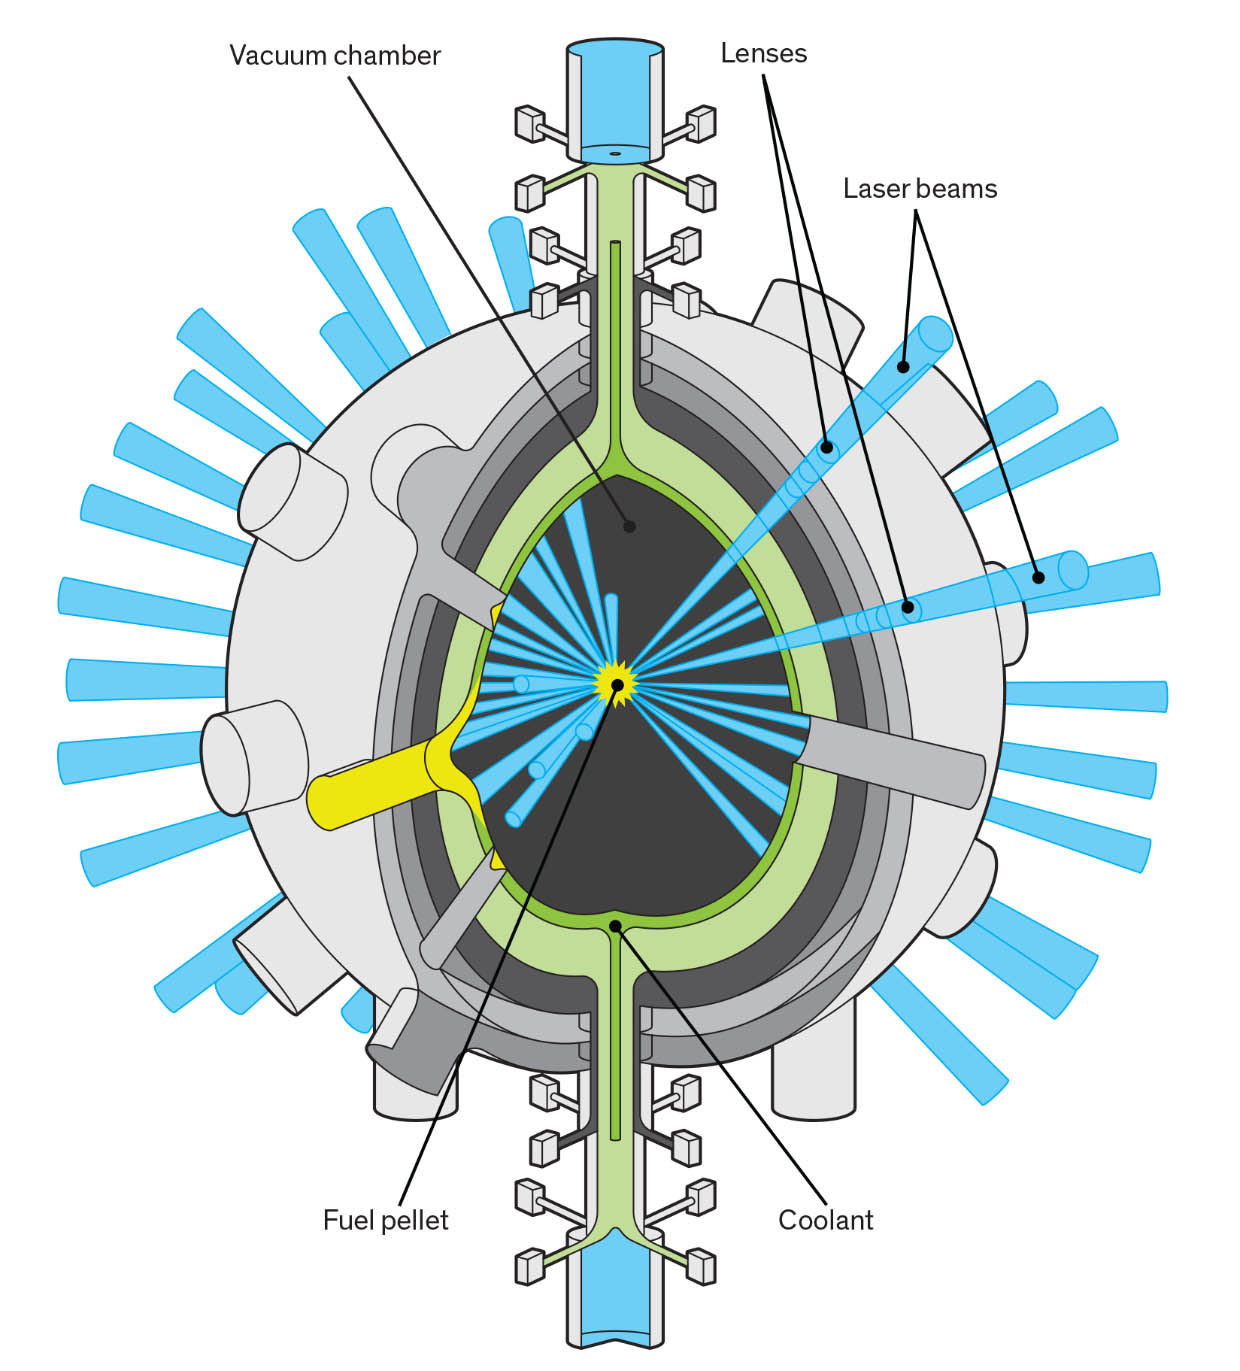
\includegraphics[width=\textwidth]{icf}}
			{\tiny
				Illustration by~Chris Philpot, courtesy of IEEE~Spectrum.
			}

			\column{0.55\textwidth}
			\begin{itemize}
				\item Designing next-gen Inertial Confinement Fusion (ICF)
					facility.

				\item \alert{Fueling} is an important consideration of
					every design.

				\item Require fuel of 2~varieties:
				\begin{itemize}
					\item Deuterium ($^2$H) -- abundant in naturally-sourced water.
					\item Tritium ($^3$H) -- extremely rare, \alert{produced
						\textit{in-reactor}.}
				\end{itemize}
				\item
					How do we find balance between $^3$H~fuel produced and
					consumed?
			\end{itemize}
		\end{columns}
\end{frame}

\begin{frame}
	\frametitle{Problem Description}
	Tritium breeding blankets convert neutron radiation to tritium fuel:
	\begin{align*}
		\isotope[1][0]{n} + \isotope[6][3]{Li} \rightarrow \isotope[3][1]{H} +
		\isotope[4][2]{He}
		\qquad\qquad
		\isotope[1][0]{n} + \isotope[7][3]{Li} \rightarrow \isotope[3][1]{H} +
		\isotope[4][2]{He} + \isotope[1][0]{n}
	\end{align*}
	\alert{Tritium breeding ratio (TBR)} = fuel bred / fuel consumed
	
	\begin{itemize}
	    \item Depends on numerous geometric and material parameters.
	    \item Evaluated precisely by OpenMC neutronics simulation \textit{Paramak}, but is computationally expensive. 
	\end{itemize}
	
	\vspace{15pt}
	
	\begin{block}{Our Challenge:}
		\begin{center}
			Produce a fast TBR function that strongly approximates Paramak, making use of the latest in surrogate modelling techniques.
		\end{center}
	\end{block}
\end{frame}

\begin{frame}
	\frametitle{Data Generation}
	We produced training and test datasets by uniform random sampling over the 7
	discrete and 11 continuous parameters of Paramak.

	\begin{columns}[T]
		\column{0.34\textwidth}

		\vspace{5pt}

		Paramak deployed on UCL's Hypatia cluster:
		\begin{itemize}
		\item Generated 1M samples.
		\item 27 days of runtime.
		\end{itemize}

		\vspace{10pt}

		2~classes of runs:
		\begin{itemize}
		\item All parameters free.
		\item Discrete fixed, continuous free.
		\end{itemize}

		\vspace{10pt}

		{\footnotesize
		Groups of fractions marked\textsuperscript{\textdagger\textdaggerdbl} are required to sum to 1.
		}

		\column{0.62\textwidth}
		\vspace{5pt}

		{\fontsize{8pt}{8pt}\selectfont
		\setlength\tabcolsep{3pt}
		\begin{tabular}{l|ll}
		\toprule
		{} & Parameter name & Domain\\
		\midrule
		\parbox[t]{2mm}{\hspace{-2pt}\multirow{12}{*}{\rotatebox[origin=c]{90}{Blanket}}}
		   & Breeder fraction\textsuperscript{\textdagger} & $[0,1]$\\
		   & Breeder \isotope[6]{Li} enrichment fraction & $[0,1]$\\
		   & Breeder material & $\{\text{Li}_2\text{TiO}_3, \text{Li}_4\text{SiO}_4\}$\\
		   & Breeder packing fraction & $[0,1]$\\
		   & Coolant fraction\textsuperscript{\textdagger} & $[0,1]$\\
		   & Coolant material & $\{\text{D}_2\text{O}, \text{H}_2\text{O}, \text{He}\}$\\
		   & Multiplier fraction\textsuperscript{\textdagger} & $[0,1]$\\
		   & Multiplier material & $\{\text{Be}, \text{Be}_{12}\text{Ti}\}$\\
		   & Multiplier packing fraction & $[0,1]$\\
		   & Structural fraction\textsuperscript{\textdagger} & $[0,1]$\\
		   & Structural material & $\{\text{SiC}, \text{eurofer}\}$\\
		   & Thickness & $[0,500]$\\
		\midrule
		\parbox[t]{2mm}{\hspace{-2pt}\multirow{6}{*}{\rotatebox[origin=c]{90}{First wall}}}
		   & Armour fraction\textsuperscript{\textdaggerdbl} & $[0,1]$\\
		   & Coolant fraction\textsuperscript{\textdaggerdbl} & $[0,1]$\\
		   & Coolant material & $\{\text{D}_2\text{O}, \text{H}_2\text{O}, \text{He}\}$\\
		   & Structural fraction\textsuperscript{\textdaggerdbl} & $[0,1]$\\
		   & Structural material & $\{\text{SiC}, \text{eurofer}\}$\\
		   & Thickness & $[0,20]$\\
		\bottomrule
		\end{tabular}
		}

    \end{columns}
\end{frame}

\begin{frame}
	\frametitle{Methodology}
		Conventional regression task -- search for a cheap surrogate $\hat{f}(x)$ that
		minimizes dissimilarity with an expensive function $f(x)$:

		\begin{itemize}
			\item
				Regression performance: mean absolute error, $\sigma$ of
				error, $R^2$, $R^2_\text{adj.}$
			\item
				Computational complexity:
				training \& prediction time / sample
		\end{itemize}

		\vspace{2em}

		2~approaches for surrogate training:
		\begin{enumerate}
			\item
				\alert{Decoupled} -- trains models from previously generated samples.
			\item
				\alert{Adaptive} -- repeats sampling \& model training, increases
				sampling density in low-performance regions.
		\end{enumerate}
\end{frame}

